\documentclass[letterpaper,10pt]{article}

\usepackage{titling}
\usepackage{listings}
\usepackage{url}
\usepackage{setspace}
\usepackage{subfig}
\usepackage{sectsty}
\usepackage{pdfpages}
\usepackage{colortbl}
\usepackage{multirow}
\usepackage{relsize}
\usepackage{amsmath}
\usepackage{fancyvrb}
\usepackage{amsmath,amssymb,amsthm,graphicx,xspace}
\usepackage[titlenotnumbered,noend,noline]{algorithm2e}
\usepackage[compact]{titlesec}
\usepackage{paratype} 
\usepackage[T1]{fontenc}
\usepackage{tikz}
\usetikzlibrary{arrows,automata,shapes,trees,matrix,chains,scopes,positioning,calc}
\tikzstyle{block} = [rectangle, draw, fill=blue!20, 
    text width=2.5em, text centered, rounded corners, minimum height=2em]
\tikzstyle{bw} = [rectangle, draw, fill=blue!20, 
    text width=4em, text centered, rounded corners, minimum height=2em]

\definecolor{namerow}{cmyk}{.40,.40,.40,.40}
\definecolor{namecol}{cmyk}{.40,.40,.40,.40}

\let\LaTeXtitle\title
\renewcommand{\title}[1]{\LaTeXtitle{\textsf{#1}}}


\newcommand{\handout}[5]{
  \noindent
  \begin{center}
  \framebox{
    \vbox{
      \hbox to 5.78in { {\bf ECE254: Operating Systems and Systems Programming } \hfill #2 }
      \vspace{4mm}
      \hbox to 5.78in { {\Large \hfill #4  \hfill} }
      \vspace{2mm}
      \hbox to 5.78in { {\em #3 \hfill} }
    }
  }
  \end{center}
  \vspace*{4mm}
}

\newcommand{\lecture}[3]{\handout{#1}{#2}{#3}{Lecture #1}}
\newcommand{\tuple}[1]{\ensuremath{\left\langle #1 \right\rangle}\xspace}

\addtolength{\oddsidemargin}{-1.000in}
\addtolength{\evensidemargin}{-0.500in}
\addtolength{\textwidth}{2.0in}
\addtolength{\topmargin}{-1.000in}
\addtolength{\textheight}{1.75in}
\addtolength{\parskip}{\baselineskip}
\setlength{\parindent}{0in}
\renewcommand{\baselinestretch}{1.5}
\newcommand{\term}{Spring 2015}

\singlespace


\begin{document}

\lecture{ 27 --- Scheduling, Idling, Priorities, and Queues }{\term}{Jeff Zarnett}

\section*{Scheduling Algorithms, Continued}

Carrying on from last time, we will examine some more scheduling algorithms.

\subsection*{Highest Response Ratio Next}

We will introduce a new measure: normalized turnaround time. This is the ratio of the turnaround time (the time waiting plus the amount of time taken to execute) to the service time (the time it takes to execute). The relative amount of time waiting is somewhat more important; we can tolerate longer processes waiting a comparatively longer period of time. The goal, then, of the HRRN strategy, is to minimize not only the normalized turnaround time for each process, but to minimize the average over all processes~\cite{osi}.

The way to calculate the response ratio, $R$, is by the following formula: $\frac{w + s}{s}$ where $w$ is the waiting time and $s$ is the service time. The service time is, as always, a guess. When it is time to select the next process to run, choose the process with the highest $R$ value. A new process will have a value of 1.0 at the beginning, because it has spent no time waiting (yet). Thus it is not that likely to get selected.

Jobs with a small $s$, i.e., short jobs, are likely to get scheduled quickly, which is still a positive. In spite of this, the HRRN approach introduces something important we have not yet had: factoring in the age of the process. The term $w$ indicates how much time a process has spent waiting. Thus, a process that has spent a long time waiting will rise in priority, over time, until it gets a turn. So processes will not starve, because even a process that is expected to have a very long $s$ will eventually have a high enough $R$ due to the growth of $w$.

We still need to have some way of estimating $s$, which may or may not be simple guessing. 

\subsection*{Multilevel Queue (Feedback)}
For the most part, until now, we have treated processes more or less equally (except when we have taken the highest priority process). While it might seem very fair, it may not be ideal for a situation where processes behave differently. A desktop or laptop has many processes running, some of which are visible to the user (foreground, or interactive processes) and some of which are not (background and batch processes). We could then apply different scheduling algorithms to different types of process.

The multilevel queue takes the ready queue and breaks it up into several queues. A process can be in one (but only one) of the queues and it is assigned to the queue based on some attribute of the process (priority, memory needs, foreground/background, et cetera). The foreground queue, for example, could be scheduled by Round Robin, and the background by First-Come, First-Served~\cite{osc}.

When there are multiple queues, we also need a way of choosing which of the queues to take from next. The policy we choose depends on goals. We might say some queues have absolute priority over others (e.g., as in the earlier highest priority, period option), or we might have time slicing amongst the queues. This could be balanced evenly (rotate through each) or give more time slices to some queues at the expense of others.

An example of this was the CTSS (Compatible TimeSharing System) that ran on the IBM~7094. The CTSS designers decided that it was ideal to give CPU-Bound processes longer blocks of time to execute so they would not have to spend so much time swapping. They set up multiple queues. In the highest priority class, a process got 1 time slice; in the next one down, a process got 2 time slices; the third class meant 4 time slices, and so on. If a process ran up against the limit of a time slice (e.g., used the full 2 time slices), it was moved down a class. So it got a lower priority, but when it did get selected to run, it was able to run with a lower chance of being interrupted~\cite{mos}.

Like a few schemes, we have seen so far, this is a ratchet: a process can move down in the priority list, but there does not appear to be a way for it to move up. So a process that needed a lot of CPU early on was going to be punished ``forever''. The designers of the system assumed that if the user pressed the Enter key, it might be a sign the process was likely to become interactive (and therefore should move up in priority). Some genius user (there's always one), figured out that by pressing the enter button repeatedly, his long running processes would finish faster. This was a bit unfair; his processes got priority over the others. But things really broke down when this individual decided to be nice: he told all his friends. And suddenly everyone was doing it and the benefit of the system was lost~\cite{mos}.

This scheduling algorithm may also be referred to as \textit{feedback}. We do not have any information in advance about how long various processes will be. Instead of being concerned with how much CPU time will be used, which requires clairvoyance or guessing, we assign priority based on the amount of CPU time assigned so far. A process that has used a lot of CPU so far gets lower priority.

\subsection*{Guaranteed Scheduling}

And now for something completely different. The idea behind guaranteed scheduling is to promise the users something and then fulfill that promise. We could promise that if there are $n$ users, each gets an equal share (1/$n$) of the CPU time. Or with $m$ processes, each process gets 1/$m$ of the CPU time.

To make this happen, the system must keep track of how much CPU time each process has received since its creation. It then considers the how this value compares to the ideal (time since creation divided by $n$). If a process has a value of 0.5, it means it has had only half the CPU it ``should'' have received. If it has a value of 2.0, it has had double. So the scheduling algorithm is then to run the process with the lowest score, trying to keep all values as close to 1.0 as we can~\cite{mos}.

\subsection*{Lottery}

The lottery is a system to give predictable results with a simple implementation. The premise is that every process gets some number of ``lottery tickets'' for each resource (e.g., CPU). When a decision has to be made, a lottery ticket is selected at random. The process that holds that ticket gets that resource. This system provides some clarity; if a process has priority $p$, what does that mean? If a process has a fraction $f$ of the total tickets, then we can expect that process to get about $f$\% of the resource. When a process is created or terminates this may increase or decrease the number of tickets, or result in their redistribution~\cite{mos}. 

More important processes are given more tickets and have, therefore, a higher chance of winning. If there are 100 tickets outstanding, if a process has 25 of them, it has a 25\% chance of winning any given draw. To increase a process's chance of winning, give it more tickets. To decrease it, give it fewer. Unlike in the real lottery, though, there is always a winner. There are no ``unpurchased'' tickets and we can choose only a ticket that someone is holding.

Co-operating processes may be permitted to exchange tickets. A client that sends a request to a server might then give all its tickets to the server, increasing the chance the server gets the resources to run next~\cite{mos}.

This is a lot less overhead than guaranteed scheduling. We do not have to keep track of how much of the resource a process has received. Assuming that the lottery system is sufficiently random, over time the resource allocation will tend towards the proportions of the tickets each process holds. If process $A$ has 20\% of the tickets, $B$ has 30\%, and $C$ has 50\%, then the CPU will be given to the processes in approximately a 20:30:50 ratio, as expected. Of course, random number generation is a small struggle for computers, though the complexity of this is not something we want to examine here.


\section*{The Idle Task}

Sometimes our scheduling algorithm cannot produce a new process to run next because there is, quite frankly, nothing to do. The actual implementation of the idle thread may vary across different systems. In some cases it is just repeatedly invoking the scheduler; in others it does a bit of useless addition; or it might just be a whole bunch of \texttt{NOP} instructions. With truly nothing to do, the CPU can be told to halt or switch to a lower power state. Whatever it actually ``does'', the idle thread never has any dependencies on anything else and is always ready to run.

Since the idle thread does not necessarily do much, why have it? It prevents having special cases in the scheduler, first of all. It also provides some accounting information about how much of the time the CPU is not doing anything. In fact, a lot of the time on the desktop or laptop, task manager will tell you that ``System Idle Process'' is taking up a large percentage of the CPU. Because you are more intelligent than a certain technology journalist who may or may not be named John Dvorak, you will recognize that this just means the CPU is not doing anything; it does not mean that some mysterious system process is using up all your CPU's time.

Saving power by shutting down (parts of) the processor seems like a nice savings of energy (and potentially increases battery life). On the other hand, time when the CPU is doing nothing might potentially be put to use. There are usually some accounting and housekeeping tasks that the CPU can be doing when it has nothing else. For example, the OS could collect statistical data, or defragment the hard drive (something we will look at).

\section*{Bumping the Priority}
Sometimes we get into a situation called a \textit{priority inversion}. This is what happens when a high priority process is waiting for a low priority process. Suppose that $P_{1}$ is high priority and is blocked on a semaphore, while $P_{2}$ is in its critical section. As $P_{2}$ is low priority, it might be a long time before $P_{2}$ is selected again to run and can finish and exit the critical section. So $P_{1}$ cannot run, because it is blocked, and it could be blocked for a very long time. In the meantime, other processes with lower priority than $P_{1}$ (but higher than $P_{2}$) carry on execution. Having $P_{1}$ waiting for the lower priority processes is rather undesirable.

The solution is \textit{priority inheritance}. The right thing to do is to bump up the priority of $P_{2}$, temporarily, to be equal to that of $P_{1}$, so that $P_{1}$ can be unblocked as quickly as possible. To generalize, a lower priority process should inherit the higher priority if a higher priority process is waiting for a resource the lower priority process holds. So $P_{2}$ will get selected, will execute and exit the critical section. Its priority then falls down to normal, meaning $P_{1}$ will be selected and may continue.

A famous case of priority inversion took place on the Mars Pathfinder rover. In short, a low priority task would acquire a semaphore, locking the information bus. A high priority task also needed that bus. There was, finally, a medium priority task for communication, which ran for a long time. If the low priority task had the bus, the high priority task was blocked; the medium priority task would be selected to run. While that happened, the low priority task could not finish and release the semaphore. Accordingly, the high priority task was stuck waiting. After a specified period of time, the system assumed the high priority task was stuck and its deadlock resolution strategy was armageddon: total system reboot (resulting in the loss of some data). 

The Pathfinder solution was to enable priority inheritance on the information bus semaphore. This meant that the low priority task would get a higher priority than the communication task and would run to completion; then the high priority task would be able to run and the system would not assume a deadlock had occurred. It was, to a certain extent, fortunate that this option was built into the system at all and needed only to be turned on. Doing a major software update on a system that is located \textit{on another planet} is not quite the same as installing Windows updates on Patch Tuesday.



\section*{Queueing Analysis (or: Oh no! Math!)}
Given the various scheduling routines, we can do an analysis of the effectiveness of some of them. We will assume that processes arrive according to a Poisson distribution (that is to say, they arrive randomly... let's not get dragged into a debase about the various distributions), and we have exponential service times. 


Note that any scheduling relationship that chooses the next item without caring how long it will run (the expected service time) obeys this relationship~\cite{osi}:

\begin{center}
	$\dfrac{T_{r}}{T_{s}} = \dfrac{1}{1 - \rho}$
\end{center}

where: $T_{r}$ is the turnaround time (waiting plus execution); $T_{s}$ is the service time (average time in running state); and $\rho$ is the processor utilization.

This includes priority-scheduling, where the priority is assigned by some means other than based on their (predicted or known) execution times. If we do make a distinction based on the expected service times, then we get some meaningful results. In our scenario, we will have two different priority classes (``high'' and ``low'', how exciting) with different service times. Preemption, in this context, means that a low priority process will be interrupted as soon as a higher priority process is ready. See the table below:

\begin{center}
	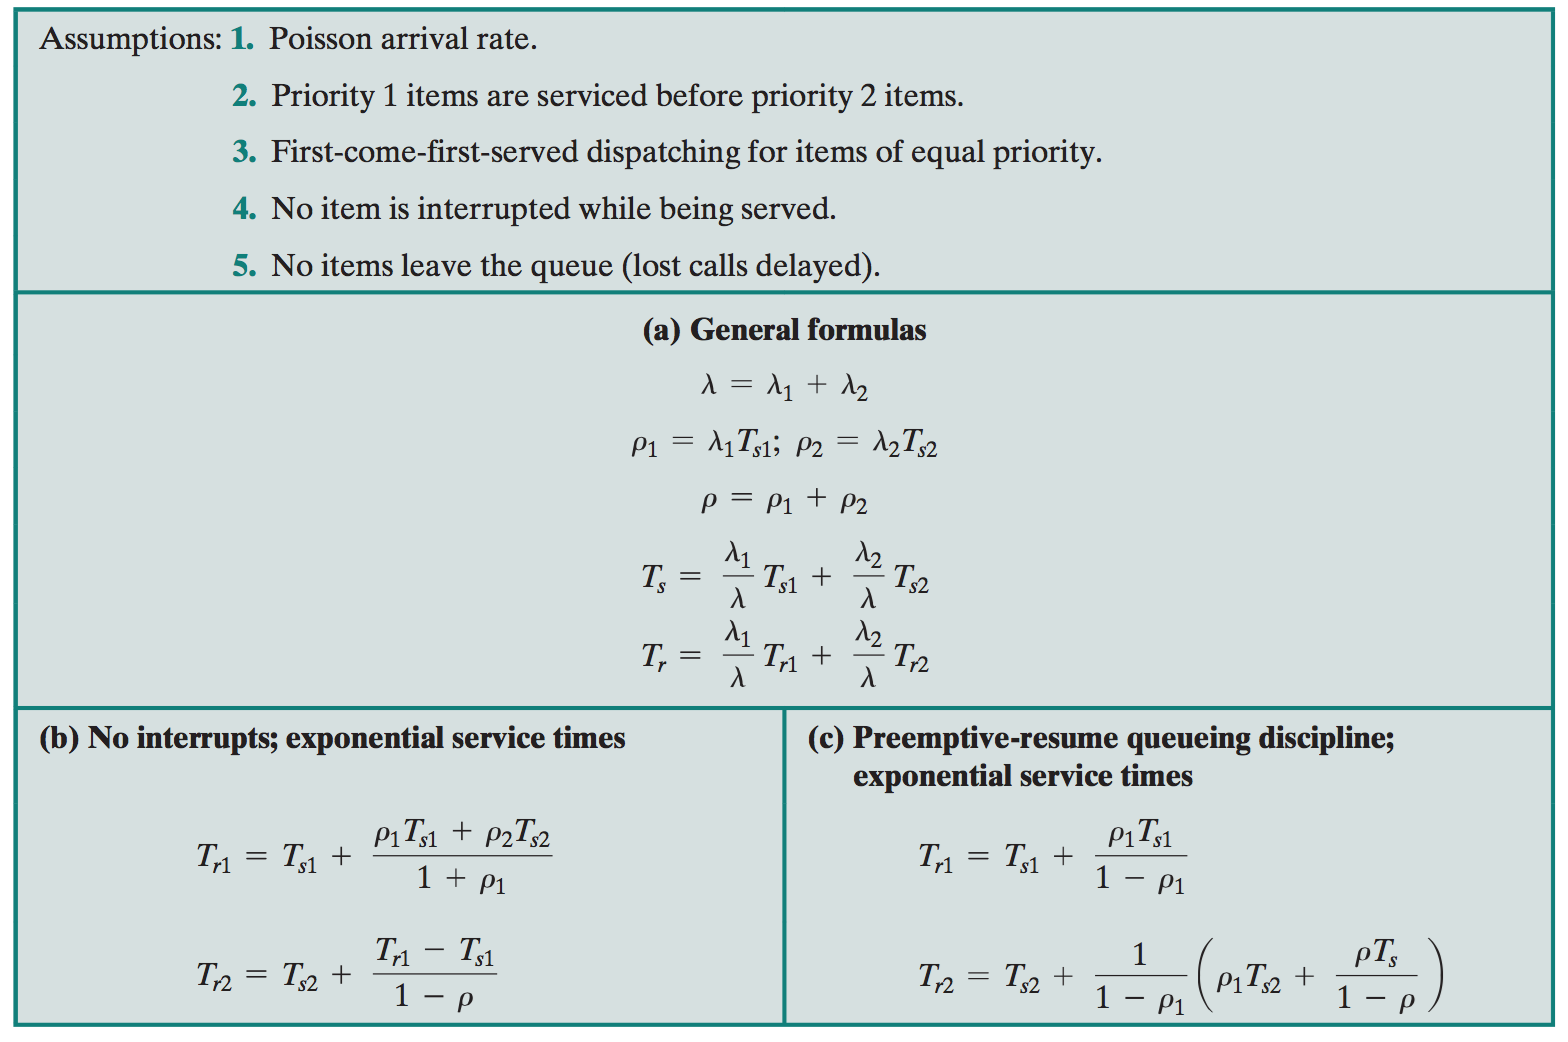
\includegraphics[width=\textwidth]{images/queue-formulae.png}\\
	Formulae for Single-Server Queues with Two Priorities~\cite{osi}.
\end{center}

Let us assume we have an equal number of arrivals between high and low priorities and that low priority tasks take about five times as long as high priority tasks. Let us look at the overall result, and then break it down into the response times for shorter processes and longer processes.

\begin{center}
	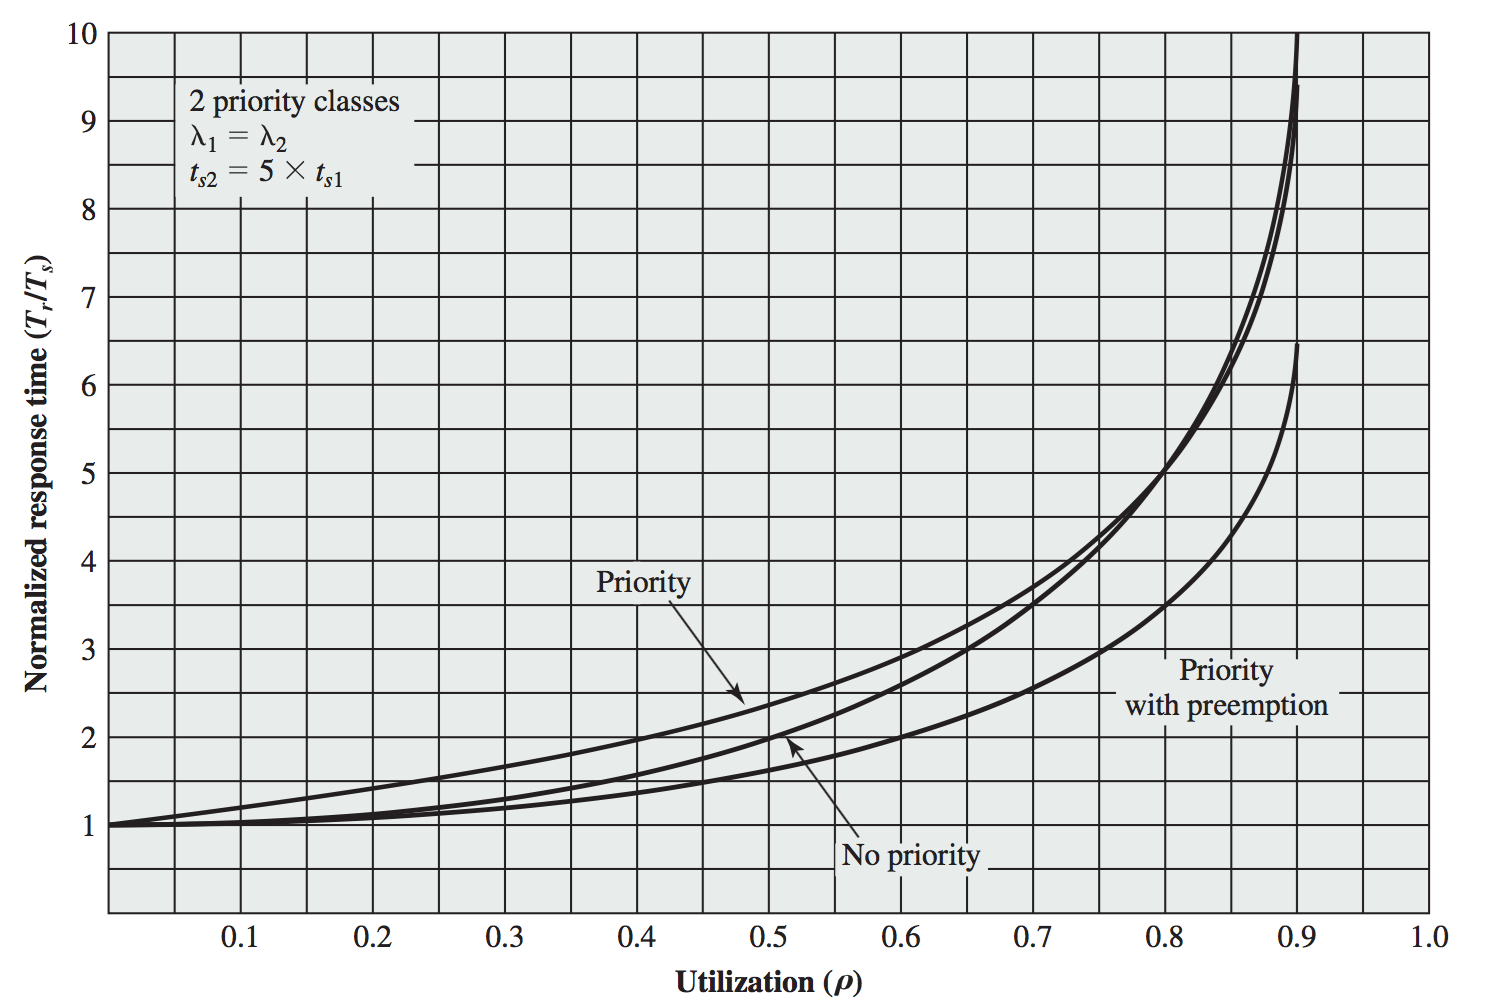
\includegraphics[width=0.63\textwidth]{images/overall-response-time.png}\\
	Overall normalized response time~\cite{osi}.
\end{center}

\vspace{-2em}

\begin{center}
	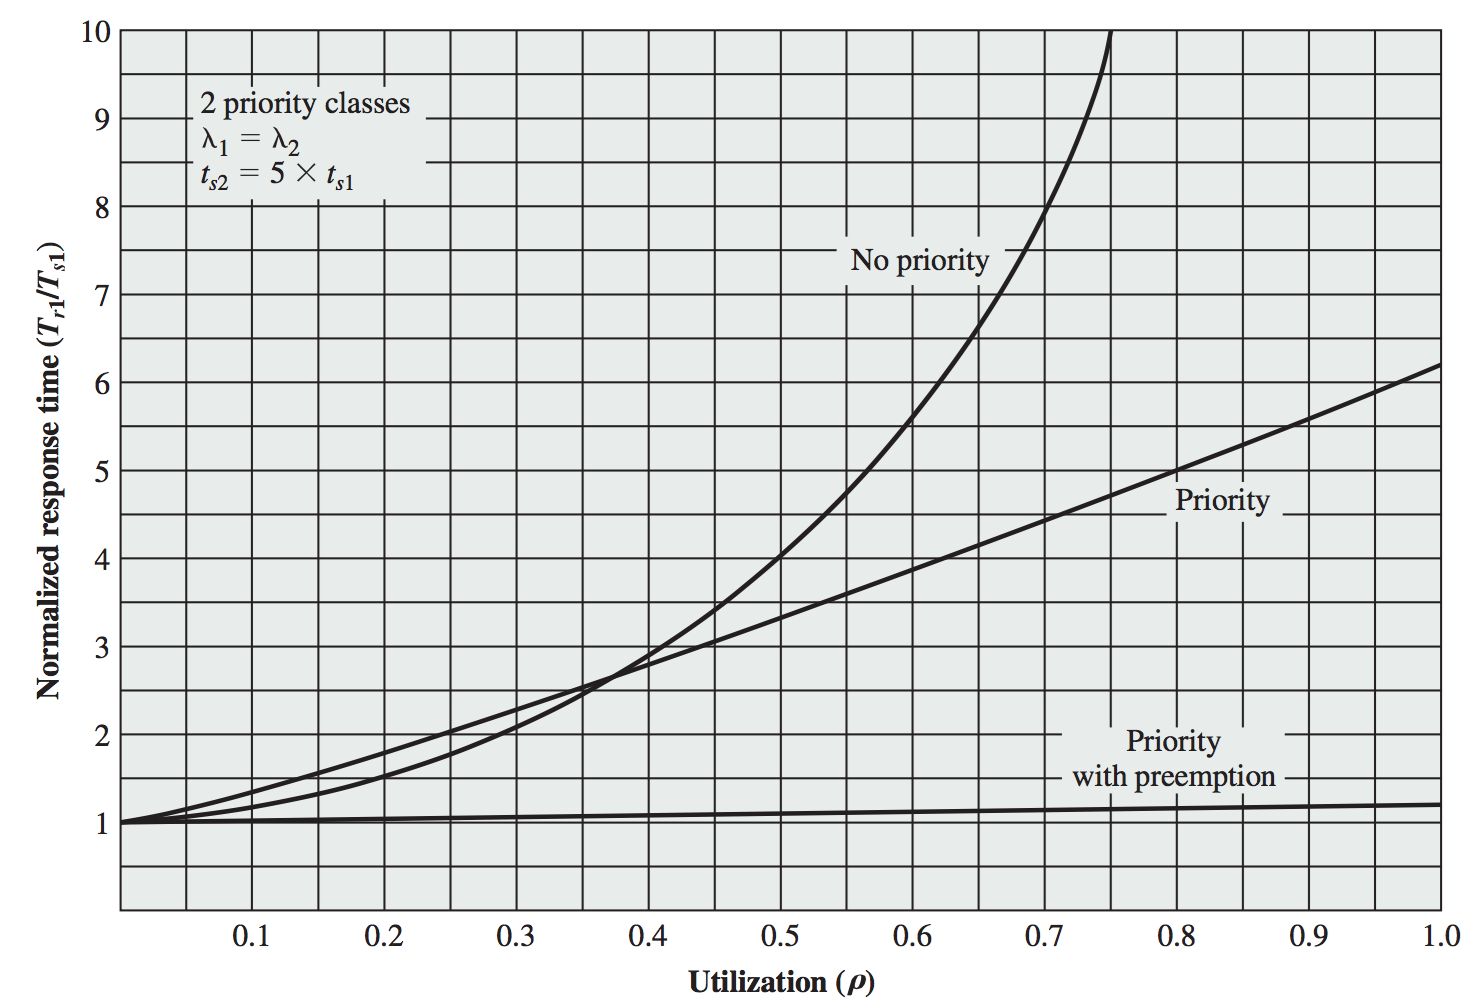
\includegraphics[width=0.63\textwidth]{images/shorter-response-time.png}\\
	Shorter process normalized response time~\cite{osi}.
\end{center}

\vspace{-2em}

\begin{center}
	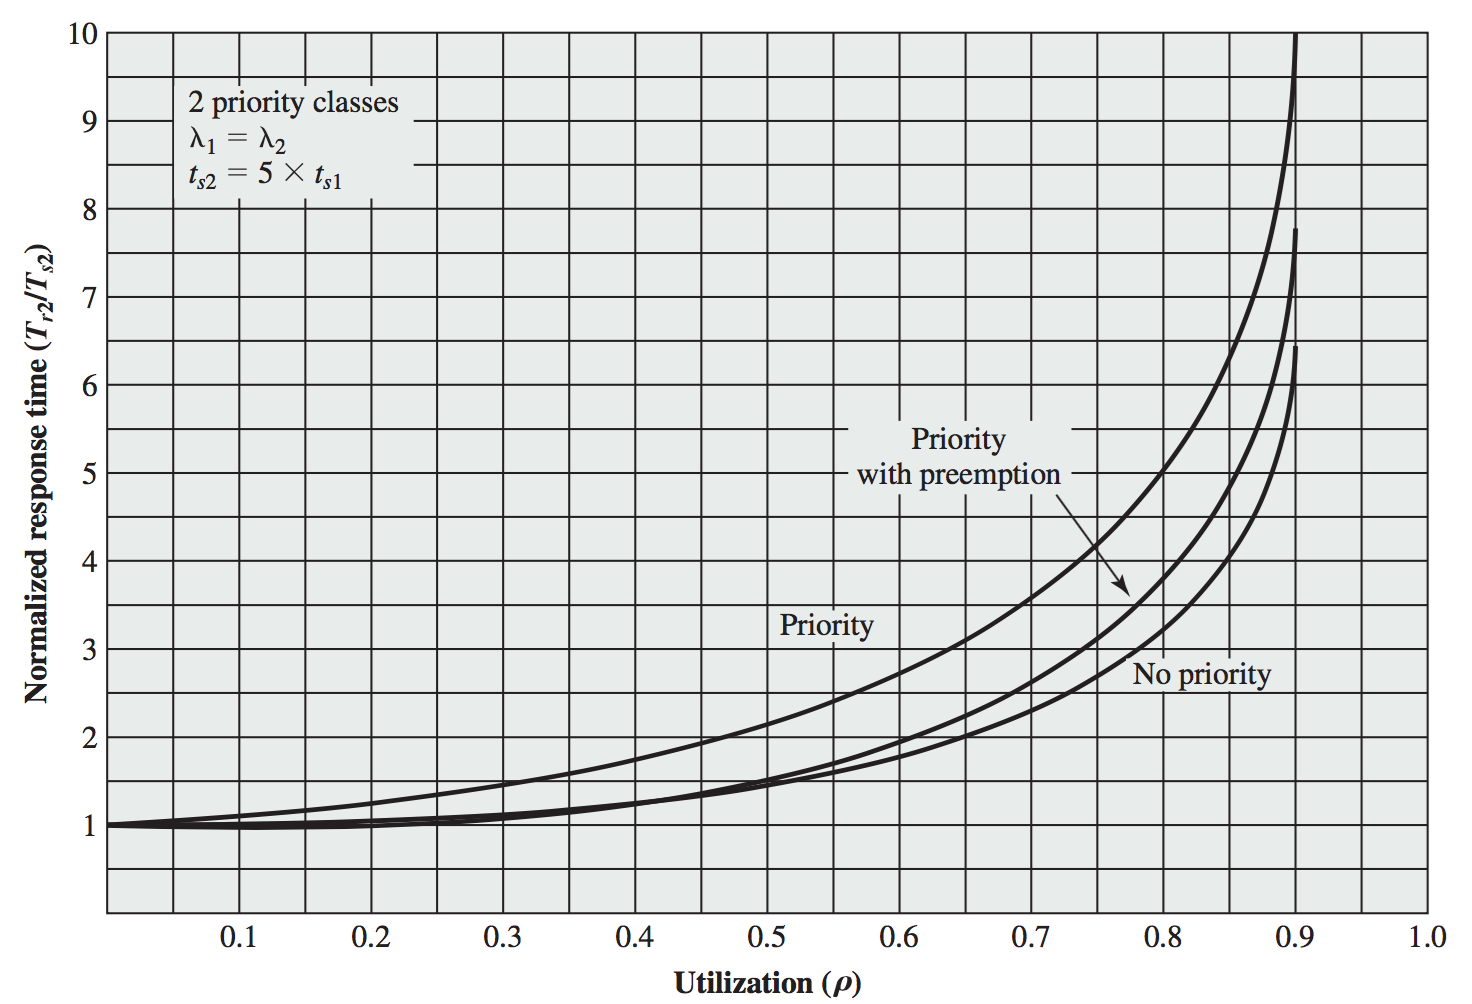
\includegraphics[width=0.63\textwidth]{images/longer-response-time.png}\\
	Longer process normalized response time~\cite{osi}.
\end{center}

\paragraph{Simulation Modelling.} Rather than just guessing about what strategy of scheduling is most effective, let us do some studies. A simulation as described in~\cite{fink} involved 50~000 processes with an arrival rate of $\lambda = 0.8$ and $T_{s} = 1$. Thus the assumption is that processor utilization $\rho$ is also 0.8. Each process is grouped into service time percentiles of 500 processes. The 500 processes with the shortest service times make the first percentile, and so on. Let us see the turnaround and waiting times, according to the simulation:

\begin{center}
	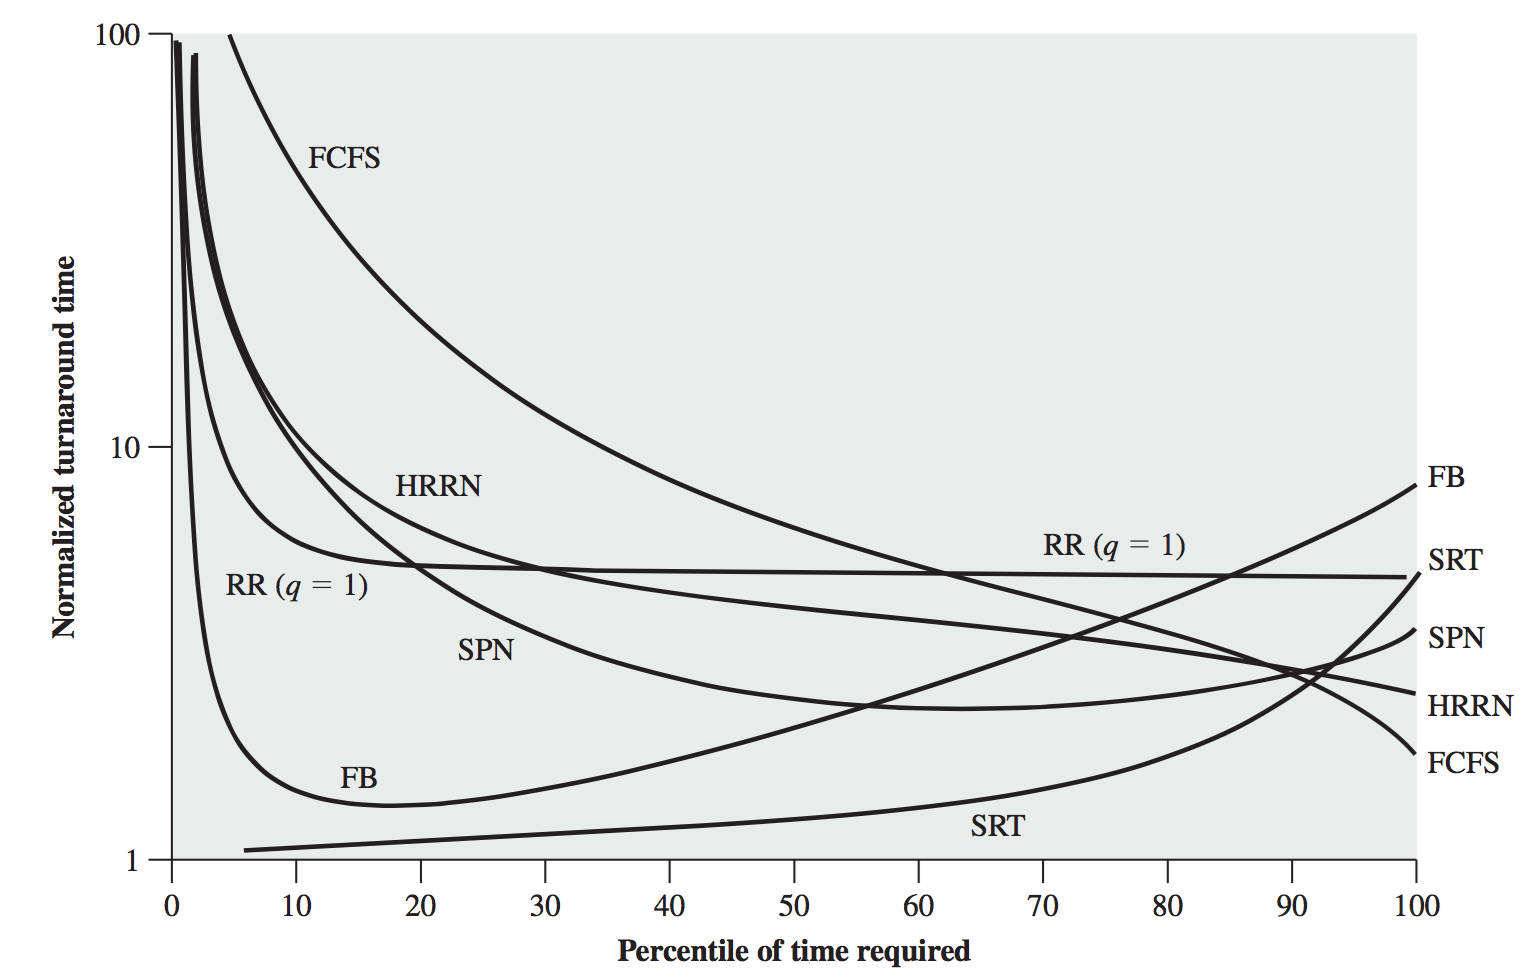
\includegraphics[width=0.85\textwidth]{images/turnaround-time.png}\\
	Turnaround time simulation result~\cite{osi}.
\end{center}

\begin{center}
	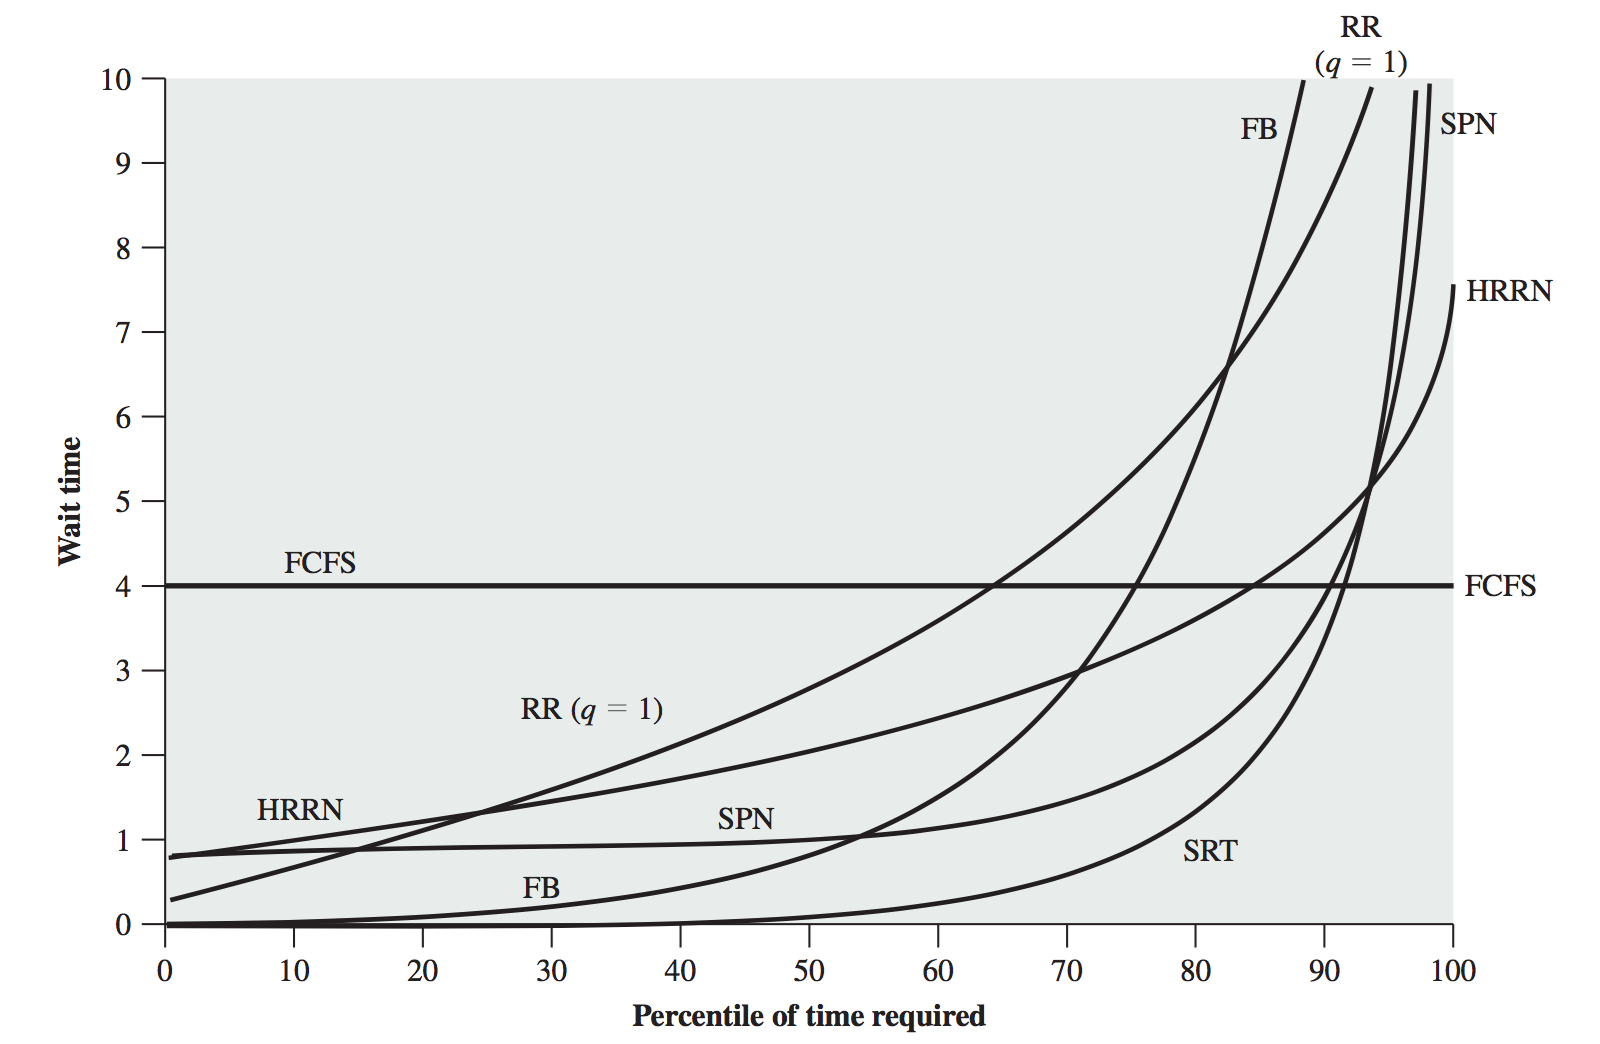
\includegraphics[width=0.85\textwidth]{images/wait-time.png}\\
	Waiting time simulation result~\cite{osi}.
\end{center}


\bibliographystyle{alpha}
\bibliography{254}


\end{document}